\section{Primeros pasos}
Lo que vamos a hacer es seguir los pasos de la página de Quetzalcoatl en el apartado de Raspberry Pi OS, al cual se puede acceder \href{https://quetzalcoatl.fciencias.unam.mx/taller-de-robotica/index.php/recursos-para-organizadores/raspberrypi-os-para-el-taller/}{acá}.

Debemos de descargar un archivo comprimido .tar.gz dando click en la palabra Jazzy (que se muestra en la siguiente figura) de la página.

\begin{figure}[H]
    \centering
    \makebox[\textwidth][c]{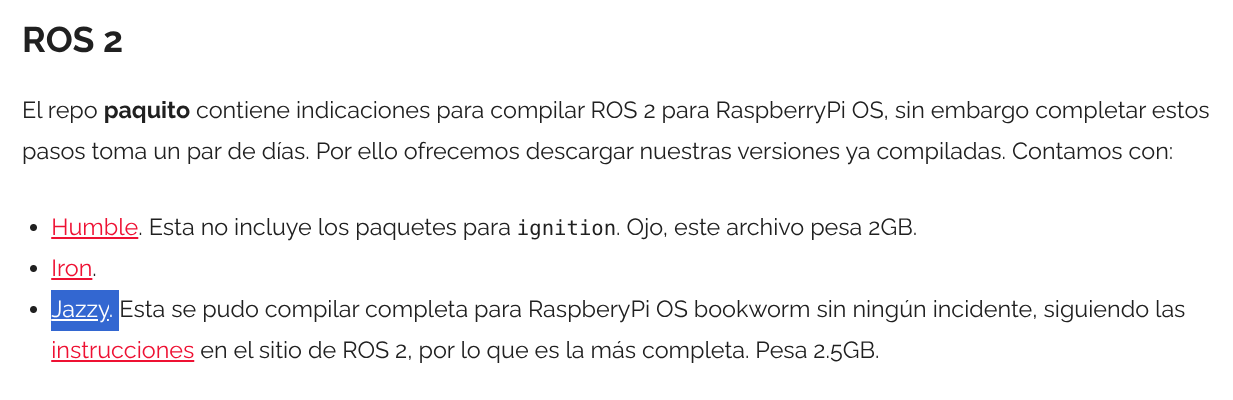
\includegraphics[width=0.8\textwidth]{imagenes/targzjazzy.png}}
    \caption{Dar Click en Jazzy para obtener el ROS compilado para Raspberry}
    \label{fig:mi_imagen}
\end{figure}

En la raspberry pi, en la ruta del usuario, se debe descomprimir el archivo descargado anteriormente con el comando \texttt{tar -xzvf archivo.tar.gz}.

\begin{center}
    \begin{Verbatim}[gobble=4]
        paquito@raspberrypi:~ $ tar -xzvf archivo.tar.gz
    \end{Verbatim}
\end{center}

Ahora, vas a tener una nueva carpeta llamada \texttt{ros2\_jazzy} dentro de la carpeta del usuario paquito. Esa carpeta ya es ROS, con esa carpeta ya tienes instalado ROS en la raspberry. Cuando instalamos ROS en una computadora normal (no raspberry) con ubuntu, la instalación de ROS se hizo en la carpeta \texttt{jazzy} en la ruta \texttt{/opt/ros/}, es decir, en nuestras computadoras tenemos a ROS instalado en \texttt{/opt/ros/jazzy/}. Sin embargo, la raspberry tiene instalado ROS en \texttt{/home/paquito/ros2\_jazzy}. Por tanto, para activar el underlay en la raspberry, debemos de escribir el siguiente comando: \texttt{source ~/ros2\_jazzy/install/local\_setup.bash}.    

Para no tener que activar el underlay todo el tiempo en la raspberry pi, vamos a guardar el comando de activación de underlay en el archivo \texttt{~/.bashrc}, para hacerlo, ejecutaremos el siguiente comando:\\\verb|echo "source ~/ros2_jazzy/install/local_setup.bash" >> ~/.bashrc|

\begin{center}
    \begin{Verbatim}[gobble=4]
    paquito@raspberrypi:~ $ echo "source ~/ros2_jazzy/install/local_setup.bash" \
    >> ~/.bashrc
    \end{Verbatim}
\end{center}

Para activar overlays, va a ser exactamente igual que en nuestras pc's. En la carpeta del espacio de trabajo, ejecutar \texttt{source install/local\_setup.bash}.